\section {Testes e Resultados}
\label{sec:resultados}

Os requisitos centrais das entregas realizadas neste trabalho eram sobre melhorar o desempenho das páginas de visualização e de edição do texto participativo.
Sendo assim, os testes de carga serão executados para medir quantitativamente os resultados obtidos pelas modificações realizadas na ferramenta de textos participativos do Brasil Participativo que visaram o ganho de desempenho.

É importante observar que as funcionalidades de \textit{parsing} de texto do usuário através do comando copiar e colar são completamente novas na plataforma, o que impossibilita um comparativo.

Para a execução dos testes, será utilizada a ferramenta de linha de comando \textit{Apache HTTP Server Benchmarking Tool} (ApacheBench).
Os testes serão executados em um computador com sistema operacional Linux, distribuição Ubuntu 24.04.2 LTS. As configurações de \textit{hardware} podem ser vistas na Tabela \ref{tab:especificacao-hardware-de-teste}.
Os testes utilizarão a aplicação do Brasil Participativo com execução em modo produção.
O protocolo utilizado será HTTP, e o próprio \textit{Rails} servirá os \textit{assets}.
O \textit{web-server Puma} será executado em \textit{single mode} com cinco \textit{threads}.

\begin{table}[h]
	\centering
	\caption{Especificação do hardware de teste}
	\label{tab:especificacao-hardware-de-teste}
	\begin{tabular}{cc}
    \toprule
    \textbf{Processador} & AMD Ryzen 5 7430U (6 Cores/ 12 Threads) \\
    \textbf{Placa de Vídeo} & Radeon Graphics 2GB (Integrado) \\
    \textbf{Memória RAM} & 24 GB DDR4 \\
		\bottomrule
	\end{tabular}
\end{table}

Os testes consistirão em submeter sob carga as páginas de visualização e edição do texto participativo.

Serão levantados dados para comparação com a realidade do cotidiano e os resultados dos testes apresentados pelo ApacheBench, trazendo a noção do impacto causado pelas modificações realizadas. Para trazer variabilidade nos testes, serão executados tanto os testes com volumetria de parágrafos histórica, quanto com volumetria de parágrafos extremas.

Para ambos os cenários de teste, cada parágrafo terá seu conteúdo preenchido com um texto de exemplo "\textit{Lorem Ipsum}" de 563 caracteres cada. O conteúdo utilizado será:

\textit{Lorem ipsum dolor sit amet, consectetur adipiscing elit. Sed in odio non mi auctor commodo. Aenean consequat metus massa, eget vulputate nibh suscipit vitae. Aliquam sagittis vel odio eleifend posuere. Curabitur hendrerit est elit, ac hendrerit nulla laoreet sit amet. Proin dictum tempor vulputate. Etiam cursus, quam sed cursus laoreet, dui nisi efficitur quam, at maximus dui nibh et velit. Curabitur ullamcorper ligula vitae mauris cursus rhoncus. Suspendisse laoreet felis euismod lorem accumsan, sit amet imperdiet mauris laoreet. Fusce vel tristique felis.}

A ideia central é checar o quão bem estas páginas da plataforma possivelmente operarão no dia-dia e em cenários de alta demanda.
Para os cenários extremos, será adotada a volumetria de 2 mil parágrafos por texto participativo, e 10 administradores utilizando a ferramenta paralelamente.

A versão anterior às modificações descritas neste trabalho utilizada para comparação nos testes é a \textit{tag} 1.5.0, que está disponível no respositório oficial do Brasil Participativo.

\subsection {Teste de Carga de Visualização do Rascunho}

\subsubsection {Contexto}

A fim de obter um parâmetro para comparação com teste de carga da página de edição de rascunho, foi executada no ambiente produtivo do Brasil Participativo uma consulta SQL para descobrir o dia que houveram mais criações de componentes de texto participativo. A consulta considera o período entre o primeiro dia do ano de 2024 até o último dia do mês de maio de 2025, admitindo apenas componentes que foram publicados e que são textos participativos. A consulta SQL pode ser conferida na Figura \ref{fig:consulta-top-5-dia-textos-criados}, e o seu resultado é demonstrado na Tabela \ref{tab:resultado-consulta-top-5-dia-textos-criados}.

\begin{figure}[htbp]
  \centering
  \caption{Consulta SQL para classificação dos dias com maior carga de criação de textos participativos}
  \label{fig:consulta-top-5-dia-textos-criados}
  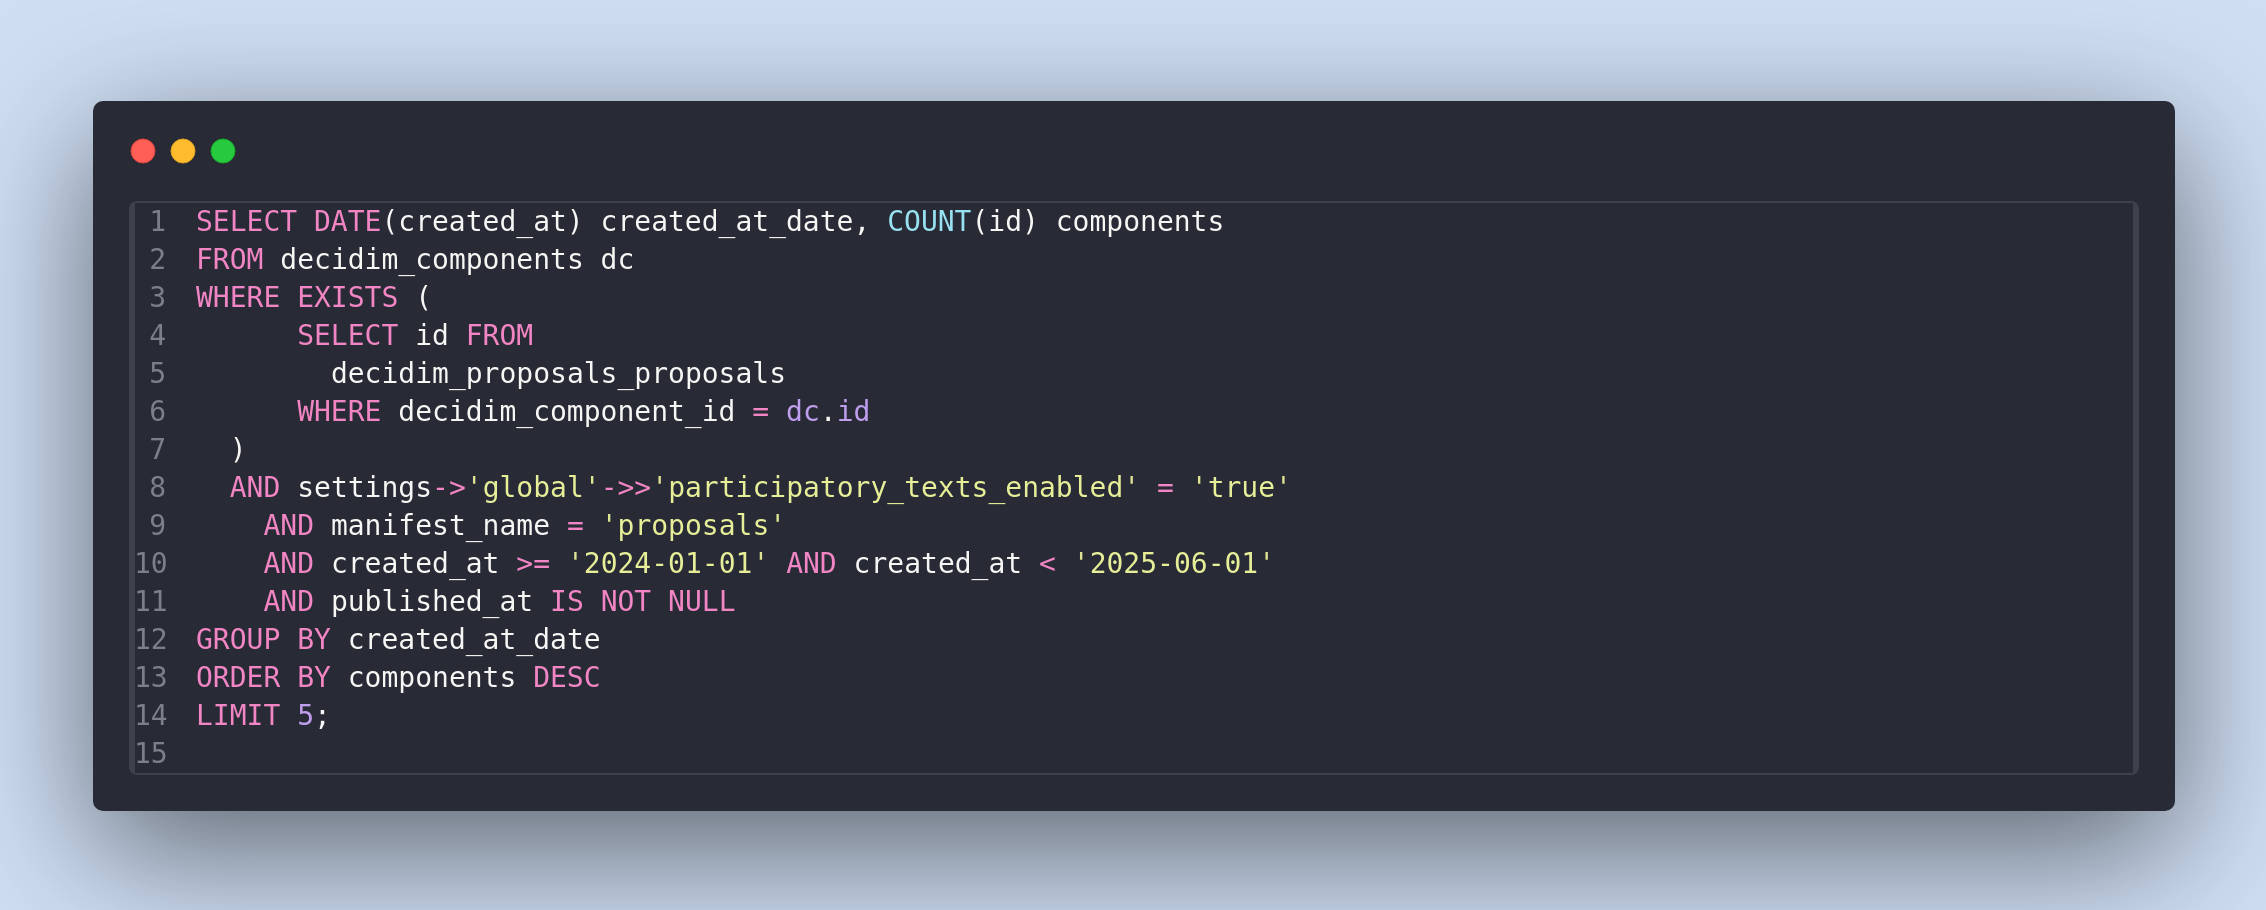
\includegraphics[width=\textwidth]{figuras/consulta-top-5-dia-textos-criados.jpg}
  \fonte{Próprio autor}
\end{figure}

\begin{table}[h]
	\centering
	\caption{Top 5 dias com maior volume de textos participativos criados}
	\label{tab:resultado-consulta-top-5-dia-textos-criados}
	\begin{tabular}{cc}
		\toprule
		\textbf{Data} & \textbf{Textos participativos criados} \\
		\midrule
    29/11/2024 & 45 \\
    30/11/2024 & 24 \\
    02/12/2024 & 17 \\
    22/01/2025 & 15 \\
    09/10/2024 & 12 \\
		\bottomrule
	\end{tabular}
  \fonte{Próprio autor}
\end{table}

No dia 29 de novembro de 2024, houveram 45 componentes de texto participativo criados na plataforma. Uma segunda consulta foi executada para descobrir a classificação dos cinco textos participativos dessa data com a maior quantidade de parágrafos. A consulta SQL pode ser conferida na Figura \ref{fig:consulta-top-textos-participativos-paragrafos}, e o seu resultado na Tabela \ref{tab:resultado-consulta-top-textos-participativos-paragrafos}. Nota-se que para essa data, o texto participativo com a maior quantidade de parágrafos foi de 124.

\begin{figure}[htbp]
  \centering
  \caption{Consulta SQL para classificação dos textos participativos com maior quantidade de parágrafos}
  \label{fig:consulta-top-textos-participativos-paragrafos}
  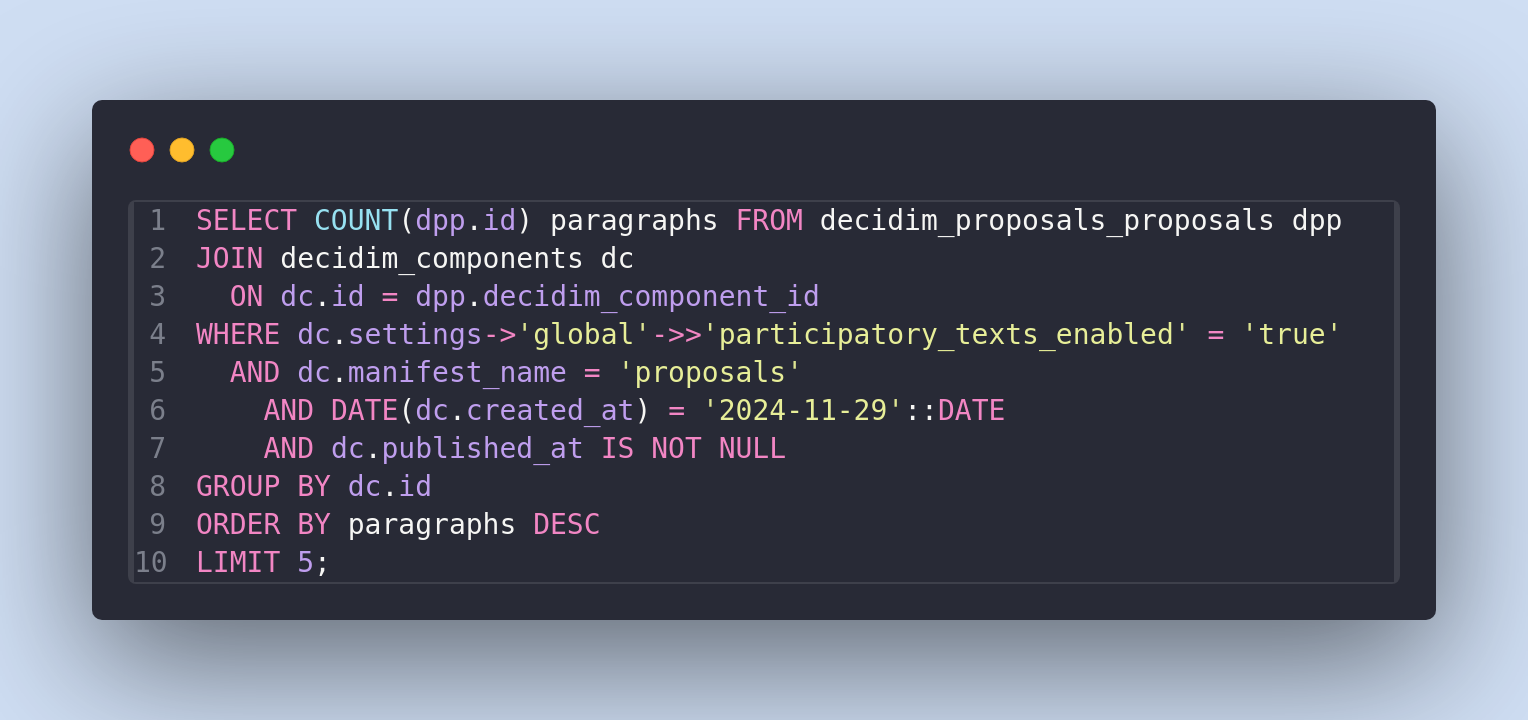
\includegraphics[width=\textwidth]{figuras/consulta-top-textos-participativos-paragrafos.png}
  \fonte{Próprio autor}
\end{figure}

\begin{table}[h]
	\centering
	\caption{Top 5 textos participativos de 29/11/2024 com maior volume de parágrafos}
	\label{tab:resultado-consulta-top-textos-participativos-paragrafos}
	\begin{tabular}{c}
		\toprule
		\textbf{Parágrafos} \\
		\midrule
    124 \\
    85  \\
    80 \\
    76 \\
    74 \\
		\bottomrule
	\end{tabular}
  \fonte{Próprio autor}
\end{table}

Com base nessas informações, será considerado um dia com pico de uso com 50 componentes sendo criados, cada um deles com 130 parágrafos.
Será levado em conta que o usuaŕio administrador possivelmente trabalha na plataforma entre os horários das nove horas da manhã até meio dia (12 horas), e das 13 horas até às 18 horas, significando uma janela de trabalho de oito horas. O que significa em aproximadamente de seis a sete componentes criados por hora.

Assumindo um possível pior cenário, também por convenção, será considerado que o administrador realiza em média no mínimo todas as cinco operações em cada parágrafo, isto é: editar, mesclar, mover, ocultar e desabilitar interações.
Para este teste será ignorado o fato de que a operação de mesclagem diminui a contagem de parágrafos em uma unidade.
A realização de cada operação acarreta na atualização da página de visualização do rascunho, portanto considerando os seis a sete componentes por hora (nesse caso será considerado sete, simplesmente), a quantidade de 150 parágrafos e as cinco operações por parágrafo, tem-se que a página de visualização do rascunho será renderizada 5.250 vezes em uma hora, ou 87 vezes por minuto, ou 1,46 vezes por segundo.

\subsubsection {Execução e Resultados}

Os testes foram realizados disparando 100 requisições com o fator de paralelismo igual a cinco, isto é, ocupando todas as cinco threads do servidor cada uma com um único usuário. Os resultados podem ser visualizados na Tabela \ref{tab:teste-carga-visualizar-rascunho}

\begin{table}[h]
	\centering
	\caption{Teste da página de edição do texto}
	\label{tab:teste-carga-visualizar-rascunho}
	\begin{tabular}{ccc}
		\toprule
		Métrica & Versão anterior & \textbf{Nova versão} \\
		\midrule
    \textbf{Tamanho da página} & 931.752 bytes & 712.295 bytes \\
    \textbf{Tempo gasto no teste} & 109 segundos & 18 segundos \\
    \textbf{Requisições por segundo} & 0,91 & 5,38 \\
    \textbf{Tempo médio por requisição} & 1.097 milissegundos & 185 milissegundos \\
		\bottomrule
	\end{tabular}
  \fonte{Próprio autor}
\end{table}

\subsubsection {Testes Extremos}

Os testes extremos foram realizados com 10 requisições com fator de paralelismo igual a 10. O número de requisições foi escolhido como 10 para garantir que os testes ocorressem em uma escala de tempo na casa de alguns minutos, evitando problemas de expiração de sessão, dado que o teste foi realizado usando um Cookie de sessão de usuário administrador extraído do navegador manualmente. O texto participativo utilizado possui 2 mil parágrafos. Os resultados podem ser conferidos na Tabela \ref{tab:teste-carga-extremo-visualizar-rascunho}.

\begin{table}[h]
	\centering
	\caption{Teste extremo da página de edição do texto}
	\label{tab:teste-carga-extremo-visualizar-rascunho}
	\begin{tabular}{ccc}
		\toprule
		Métrica & Versão anterior & \textbf{Nova versão} \\
		\midrule
    \textbf{Tamanho da página} & 14.027.611 bytes & 5.888.914 bytes \\
    \textbf{Tempo gasto no teste} & 158 segundos & 20 segundos \\
    \textbf{Requisições por segundo} & 0,06 & 0,48 \\
    \textbf{Tempo médio por requisição} & 15.837 milissegundos & 2.084 milissegundos \\
		\bottomrule
	\end{tabular}
  \fonte{Próprio autor}
\end{table}

\subsection {Teste de Carga de Visualização do Texto}

\subsubsection {Execução e Resultados}

Os testes foram realizados disparando 100 requisições com o fator de paralelismo igual a cinco. Os resultados podem ser visualizados na Tabela \ref{tab:teste-carga-visualizar-texto}. Para esse teste não se faz necessário o uso de Cookie de sessão de usuário, uma vez que a página é pública e possível de visualizar sem estar logado na plataforma.

\begin{table}[h]
	\centering
	\caption{Teste da página de visualização do texto}
	\label{tab:teste-carga-visualizar-texto}
	\begin{tabular}{ccc}
		\toprule
		Métrica & Versão anterior & \textbf{Nova versão} \\
		\midrule
    \textbf{Tamanho da página} & 437.372 & 528.236 \\
    \textbf{Tempo gasto no teste} & 455 segundos & 15 segundos \\
    \textbf{Requisições por segundo} & 0,22 & 6,61 \\
    \textbf{Tempo médio por requisição} & 4.551 milissegundos & 151 milissegundos \\
		\bottomrule
	\end{tabular}
  \fonte{Próprio autor}
\end{table}

\subsubsection {Testes Extremos}

\begin{table}[h]
	\centering
	\caption{Teste extremo da página de visualização do texto}
	\label{tab:teste-carga-extremo-visualizar-texto}
	\begin{tabular}{ccc}
		\toprule
		Métrica & Versão anterior & \textbf{Nova versão} \\
		\midrule
    \textbf{Tamanho da página} & 2.510.864 bytes & 3.239.958 bytes \\
    \textbf{Tempo gasto no teste} & 503 segundos & 16 segundos \\
    \textbf{Requisições por segundo} & 0,02 & 0,61 \\
    \textbf{Tempo médio por requisição} & 50.345 milissegundos & 1.644 milissegundos \\
		\bottomrule
	\end{tabular}
  \fonte{Próprio autor}
\end{table}

\subsection {Resultados Gerais}

As alterações abordadas neste trabalho foram devidamente incluídas no código fonte do Brasil Participativo e utilizadas no ambiente produtivo. Até o presente momento a ferramenta está sendo utilizada e posta à prova. Considera-se como um sucesso o atingimento de todos os requisitos levantados dado fato que foi realizada uma cerimonia de validação juntamente com o time de produto do Lab Livre.

\chapter {Considerações Finais}

Este trabalho teve como objetivo demonstrar a explorar uma jornada de desenvolvimento de funcionalidades levando em consideração requisitos levantados por \textit{stakeholders} e outros times, tendo como foco principal o desenvolvimento de funcionalidades com requisitos de desempenho mais rigorosos.

A metodologia adotada se baseou no desenvolvimento continuo, onde em cada ciclo de desenvolvimento novos requisitos eram priorizados e executados. A mudança de escopo, apesar de não ser o foco de detalhamento desse trabalho, foi algo presente na jornada de desenvolvimento, mas em nenhum momento foi impeditivo para realização de entregas.

Apesar do enfoque em otimização de desempenho, muitos outros tópicos relacionados ao desenvolvimento foram abordados, trazendo maior profundidade em relação às contribuições realizadas no projeto.

É esperado que a medida que a funcionalidade seja utilizada por usuários reais, correções e ajustes sejam feitos pelo time desenvolvimento do Lab Livre, trazendo maior maturidade e grau de confiança na solução.

Muitos dos tópicos aqui abordados podem vir a ser objeto de evolução futuramente, principalmente em relação a desempenho.

Sabe-se que ainda há oportunidades de desenvolvimento que potencialmente trarão melhorias de desempenho para a plataforma e para a ferramenta de textos participativos.
Como mencionado, existem diversos outros problemas de desempenho em partes específicas do sistema.

